%%%% IJCAI--ECAI 26 Supplementary Material
\typeout{IJCAI--ECAI 26 Supplementary Material}

\documentclass{article}
\pdfpagewidth=8.5in
\pdfpageheight=11in

% The file ijcai26.sty is the IJCAI style file
\usepackage{ijcai26}

% Use the postscript times font!
\usepackage{times}
\usepackage{soul}
\usepackage{url}
\usepackage[hidelinks]{hyperref}
\usepackage[utf8]{inputenc}
\usepackage[T1]{fontenc}
\usepackage[small]{caption}
\usepackage{amsmath}
\usepackage{amssymb}

\usepackage{placeins}
\usepackage{amsthm}
\usepackage{booktabs}
\usepackage[ruled,vlined,linesnumbered]{algorithm2e}
\usepackage{subcaption}
\usepackage{tabularx}
\usepackage{xcolor}
\usepackage{tcolorbox}
\usepackage{float}
\usepackage{placeins}
\usepackage[switch]{lineno}  % Required for compatibility with cached aux files

\urlstyle{same}

% PDF Info
\pdfinfo{
/TemplateVersion (IJCAI.2026.0)
}

\title{Supplementary Material: \\ "More at Stake: How Payoff and Language Shape LLM Agent Strategies in Cooperation Dilemmas"}

\date{}

\begin{document}

\maketitle

\setcounter{figure}{0}
\setcounter{equation}{0}
\setcounter{table}{0}
\renewcommand*{\thefigure}{A\arabic{figure}}
\renewcommand*{\theequation}{A\arabic{equation}}
\renewcommand*{\thetable}{A\arabic{table}}



\section{Supplement to Methodology}

\subsection{LLM Configuration}
\label{appendix:llm_config}

Table~\ref{tab:llm_config} summarizes the configuration of LLM backends used in our experiments. Following the FAIRGAME protocol~\cite{buscemi2025fairgame}, we adopt each provider's recommended default settings to reflect realistic deployment conditions.

\begin{table}[ht]
\centering
\footnotesize
\begin{tabular}{lccc}
\toprule
\textbf{Model} & \textbf{Provider} & \textbf{Temperature} & \textbf{Top\_p} \\
\midrule
GPT-4o & OpenAI & 1.0 & 1.0 \\
Claude 3.5 Haiku & Anthropic & 1.0 & 1.0 \\
Mistral Large & Mistral AI & 0.3 & 1.0 \\
\bottomrule
\end{tabular}
\caption{LLM backend configurations. Temperature and sampling parameters follow each provider's recommended defaults. While this introduces potential variability confounds in cross-model comparisons, it reflects realistic deployment conditions where practitioners use models ``out of the box.''}
\label{tab:llm_config}
\end{table}

\subsection{Payoff Scaling Examples}
\label{appendix:payoff_scaling}

For illustration, the scaled payoff matrices under the three experimental conditions are shown below. When $\lambda = 0.1$ (attenuated stakes), the row player's payoff matrix becomes:
\[
\begin{array}{c|cc}
 & \text{Option A} & \text{Option B} \\
\hline
\text{Option A} & (0.6, 0.6) & (0, 1.0) \\
\text{Option B} & (1.0, 0) &  (0.2, 0.2)
\end{array}
\]
When $\lambda = 10.0$ (amplified stakes), it becomes:
\[
\begin{array}{c|cc}
 & \text{Option A} & \text{Option B} \\
\hline
\text{Option A} & (60, 60) & (0, 100) \\
\text{Option B} & (100, 0) & (20, 20)
\end{array}
\]
The ordering $T < R < P < S$ is preserved in all cases, ensuring the strategic structure of the Prisoner's Dilemma remains unchanged while only the magnitude of incentives varies.

\subsection{Rule-Based Strategy Assignment}
\label{appendix:rule_based}

To complement the LSTM-based strategy predictions and address cases where behavioral patterns exhibit characteristics of multiple canonical strategies, we apply deterministic rule-based algorithms to identify all potential strategy labels consistent with observed action sequences. These rules encode the defining characteristics of each strategy as logical conditions on the agent's action trajectory $\mathbf{a} = (a_1, a_2, \ldots, a_T)$ and the opponent's history $\mathbf{o} = (o_1, o_2, \ldots, o_T)$.

\textbf{Always Cooperate (ALLC):} The agent cooperates in all rounds regardless of opponent behaviour.
\[
\text{ALLC} \equiv \forall t \in \{1, \ldots, N\}: a_t = C
\]

\textbf{Always Defect (ALLD):} The agent defects in all rounds regardless of opponent behaviour.
\[
\text{ALLD} \equiv \forall t \in \{1, \ldots, N\}: a_t = D
\]

\textbf{Tit-for-Tat (TFT):} The agent cooperates in round 1, then copies the opponent's previous action. To accommodate execution errors, we tolerate up to $\epsilon_{\text{noise}}$ deviations from pure TFT logic.
\[
\text{TFT} \equiv (a_1 = C) \land \left(\sum_{t=2}^{N} \mathbb{I}[a_t \neq o_{t-1}] \leq \epsilon_{\text{noise}} \cdot (N-1)\right)
\]
where $\mathbb{I}[\cdot]$ is the indicator function and $\epsilon_{\text{noise}} = 0.1$ in our implementation.

\textbf{Win-Stay-Lose-Shift (WSLS):} The agent repeats its previous action if the outcome was a Reward ($R$, mutual cooperation) or Temptation ($T_{\text{emp}}$, successful defection), and switches otherwise. The initial action can be either $C$ or $D$. Similarly, we tolerate up to $\epsilon_{\text{noise}}$ deviations.

\begin{equation*}
\begin{split}
& \text{Let } \hat{a}_t = 
    \begin{cases} 
        a_{t-1} & \text{if } (a_{t-1}, o_{t-1}) \in \{(C,C), (D,C)\} \\ 
        \neg a_{t-1} & \text{if } (a_{t-1}, o_{t-1}) \in \{(C,D), (D,D)\} 
    \end{cases} \\
& \text{WSLS} \equiv \sum_{t=2}^{N} \mathbb{I}\left[a_t \neq \hat{a}_t\right] \leq \epsilon_{\text{noise}} \cdot (N-1)
\end{split}
\end{equation*}
These rules are applied sequentially to each trajectory. A trajectory may receive multiple labels if it satisfies conditions for overlapping strategies (e.g., a short sequence of all-cooperate satisfies both ALLC and TFT). To avoid double-counting in aggregate statistics, we apply a priority ordering: pure unconditional strategies (ALLD, ALLC) take precedence over conditional ones (TFT, WSLS), reflecting their simpler generative structure. The hybrid pipeline combines these rule-based assignments with LSTM predictions: high-confidence LSTM outputs ($\tau \ge 0.9$) are retained, while ambiguous cases ($\tau < 0.9$) are supplemented with rule-based labels when applicable. In our corpus, 4.2\% of trajectories received multiple candidate labels before priority resolution. This approach ensures both coverage (via rules for unambiguous patterns) and robustness (via LSTM for noisy, complex cases).

\subsection{High-Confidence Filtering Rationale}
\label{appendix:filtering_rationale}

We employed a selective filtering approach to ensure the reliability of our LLM behavioural strategy analysis. Specifically, we focused our analysis on game instances where the predicted strategy labels for both agents exhibited prediction probabilities exceeding 0.9 (90\% confidence threshold). The decision to use high-confidence predictions is grounded in several key considerations:
\begin{itemize}
    \item \textbf{Pattern Alignment with Theoretical Strategies:} Samples with prediction probabilities above 0.9 indicate that the observed behavioural sequences of LLMs closely align with the canonical patterns defined by the four classical strategies (ALLD, ALLC, WSLS, and TFT).
    \item \textbf{Signal-to-Noise Separation:} While the probabilities are not absolute (not reaching 1.0), this is expected and attributable to inherent noise in LLM decision-making processes.
    \item \textbf{Statistical Reliability:} By focusing on high-confidence predictions, we minimize the risk of misclassification and ensure that our strategy distribution analysis reflects genuine behavioural patterns.
\end{itemize}

\subsection{Threshold Sensitivity Analysis}
\label{appendix:threshold_sensitivity}

To validate our choice of confidence threshold $\tau = 0.9$, we conducted a systematic sensitivity analysis across $\tau \in [0.3, 0.95]$ for 3-, 4-, and 5-strategy classification models. Figure~\ref{fig:threshold_sensitivity} illustrates how retention rate, average confidence, number of predictions retained, and strategy diversity vary as a function of threshold value.

\begin{figure}[ht]
    \centering
    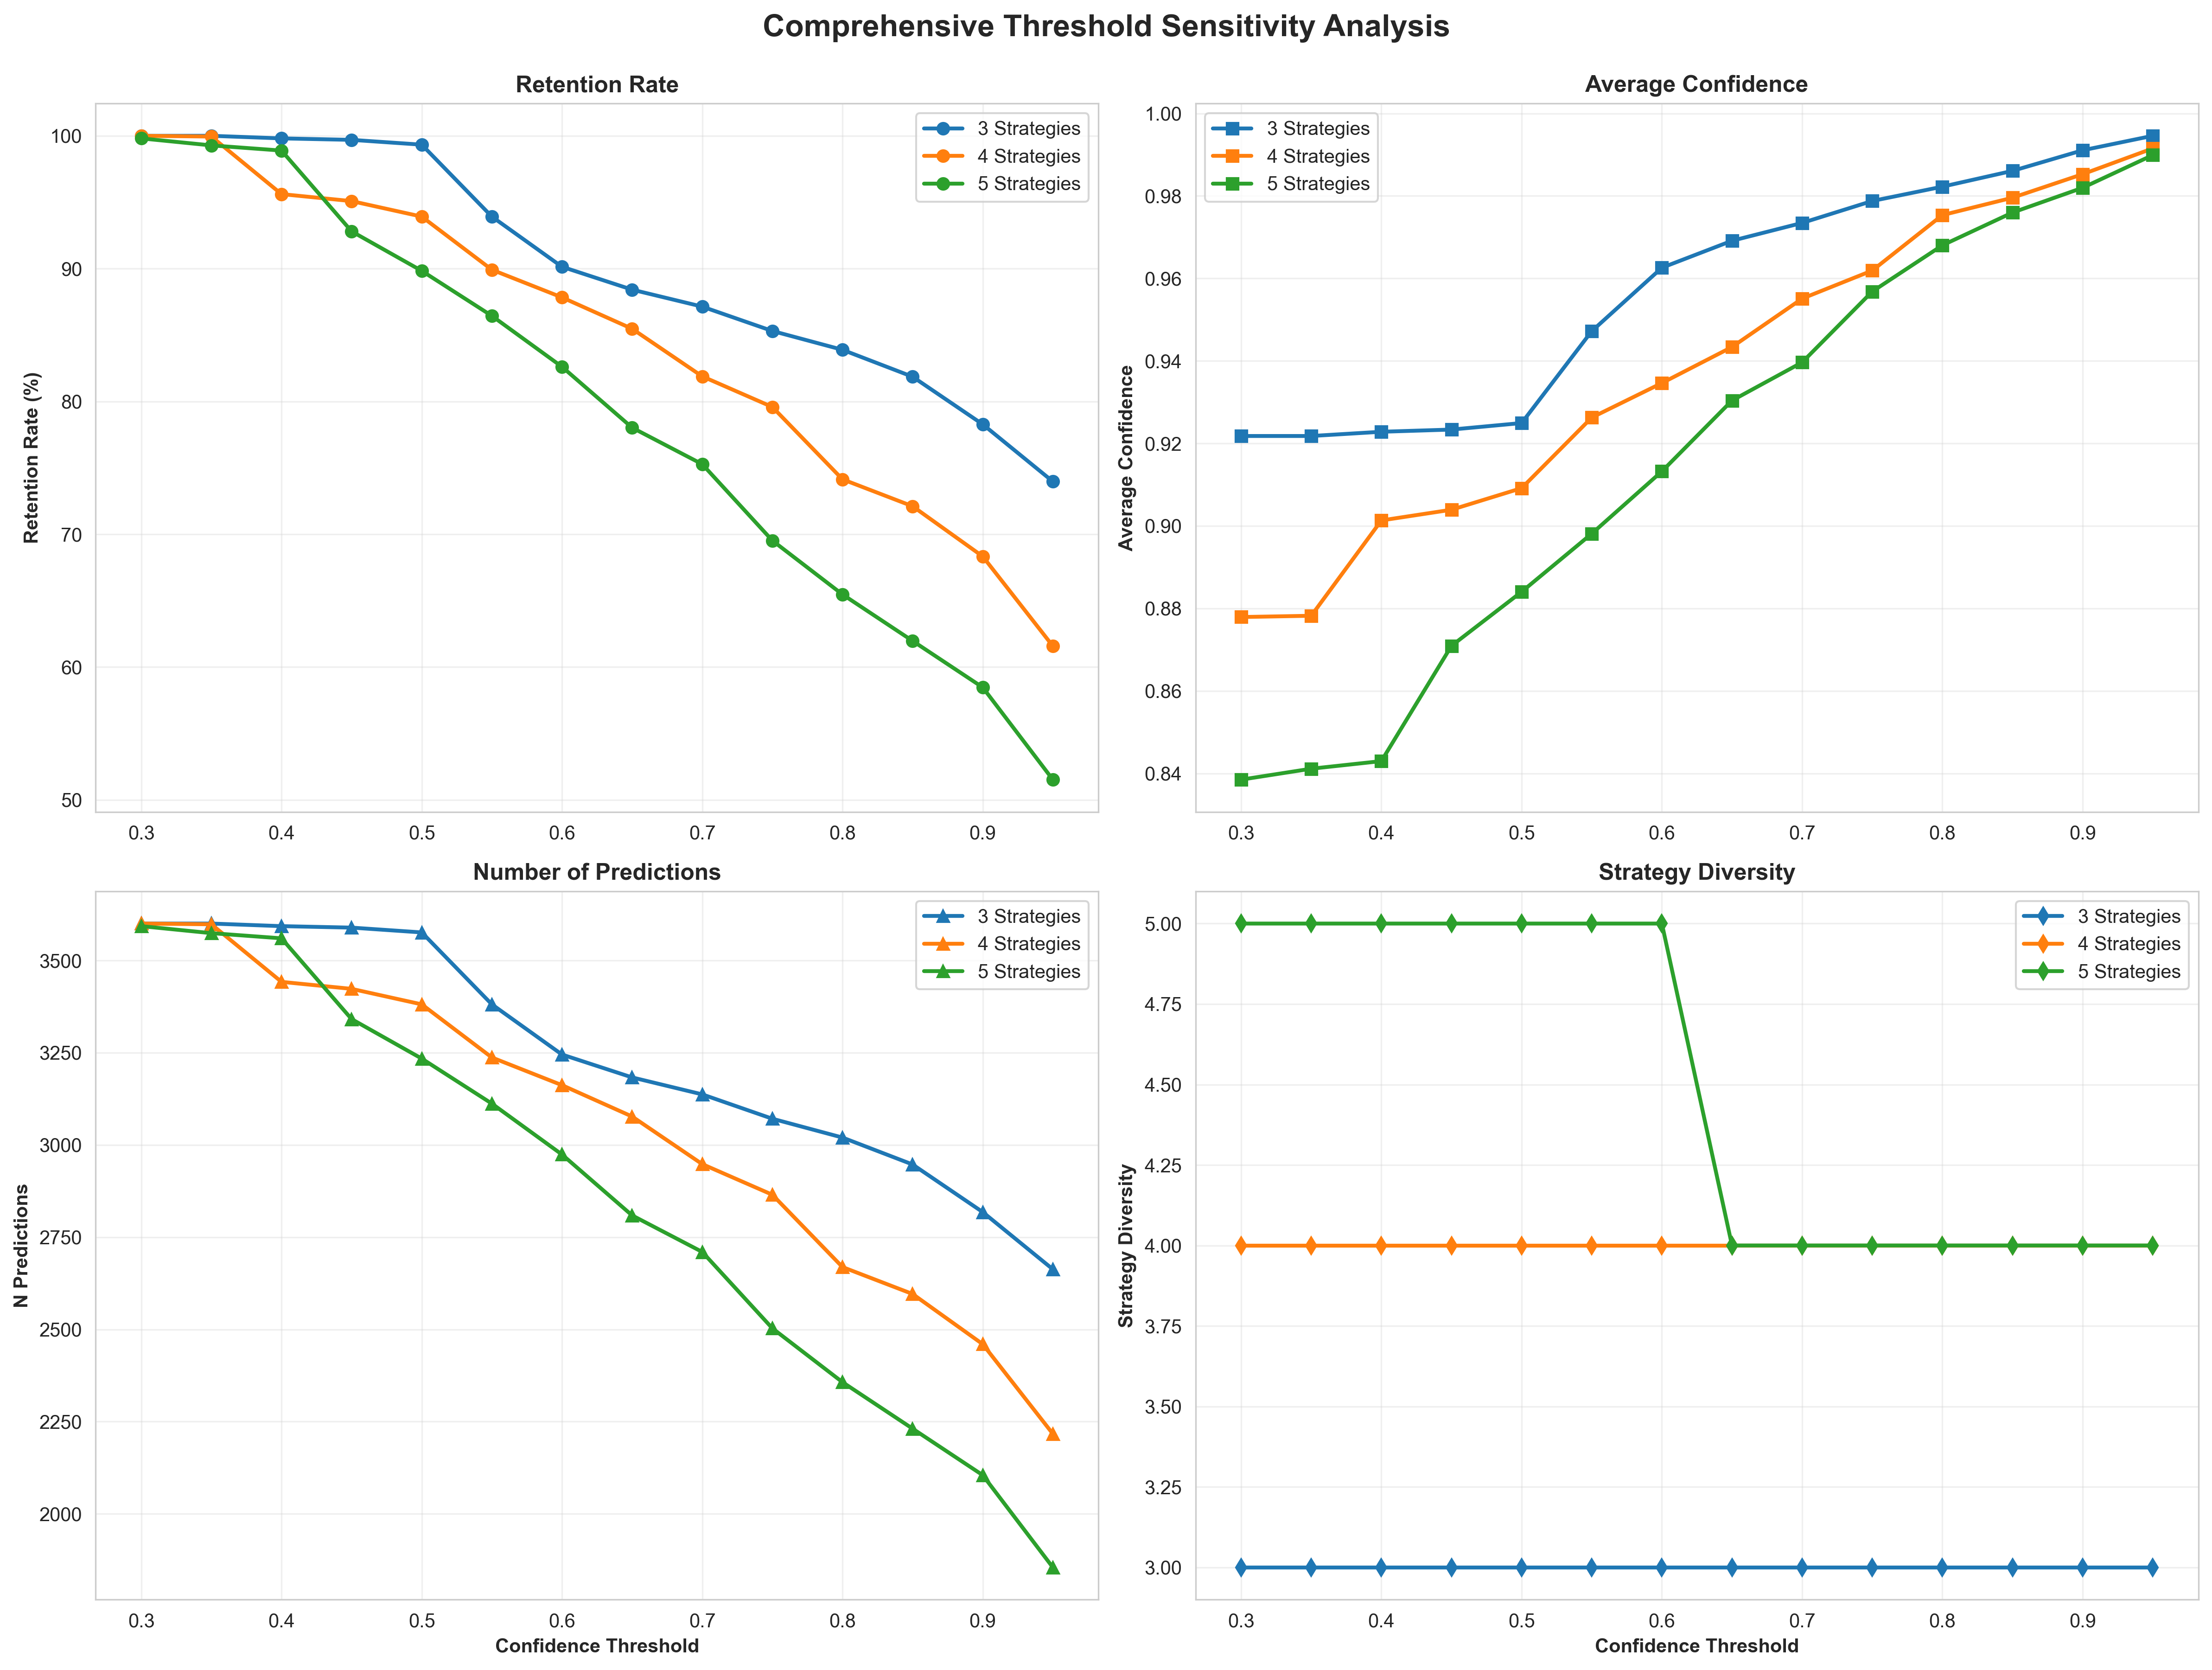
\includegraphics[width=\linewidth]{figures/8_combined_metrics.png}
    \caption{Comprehensive threshold sensitivity analysis for payoff-scaled experiments. Top row: retention rate and average confidence vs. threshold. Bottom row: number of predictions retained and strategy diversity. The 4-strategy model at $\tau = 0.9$ provides optimal balance between coverage (58.5\% retention) and reliability (avg. confidence 0.99).}
    \label{fig:threshold_sensitivity}
\end{figure}

Table~\ref{tab:threshold_comparison} summarises key metrics at $\tau = 0.9$:

\begin{table}[ht]
\centering
\footnotesize
\begin{tabular}{lccc}
\hline
\textbf{Metric} & \textbf{3-Strat} & \textbf{4-Strat} & \textbf{5-Strat} \\
\hline
Retention Rate & 78.3\% & 58.5\% & 53.2\% \\
Avg Confidence & 0.989 & 0.985 & 0.978 \\
Diversity & 3 & 4 & 4 \\
\hline
\end{tabular}
\caption{Threshold sensitivity at $\tau = 0.9$ across strategy models.}
\label{tab:threshold_comparison}
\end{table}

Key findings: (1) Retention rate decreases as strategy space expands, reflecting greater behavioral complexity; (2) Average confidence remains $>0.97$ at $\tau = 0.9$ across all models; (3) Lowering to $\tau = 0.7$ would increase retention to 75--87\% but reduce average confidence to 0.94--0.97. Our choice of $\tau = 0.9$ prioritizes classification reliability while maintaining sufficient coverage for statistical analysis.

\subsection{Model Robustness to Noise}

\begin{figure}[ht]
    \centering
    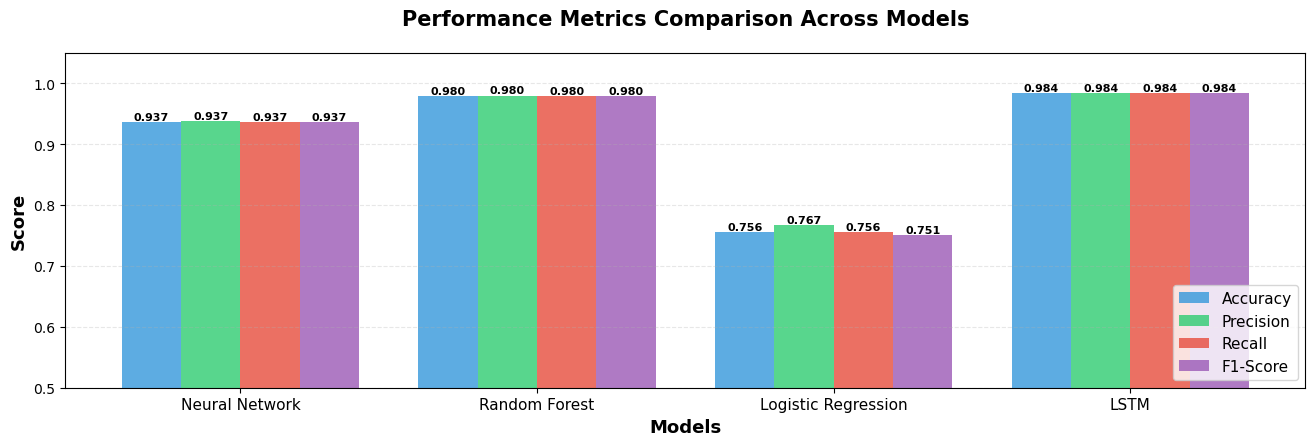
\includegraphics[width=\linewidth]{figures/model_performance_comparison.png}
    \caption{Model Robustness to Noise. Comparison of Accuracy and F1-Score between Logistic Regression, Random Forest, and LSTM on No-Noise and Noise 0.05 datasets. The LSTM demonstrates superior resilience to execution noise.}
    \label{fig:model_robustness_appendix}
\end{figure}

\begin{figure*}[ht]
    \centering
    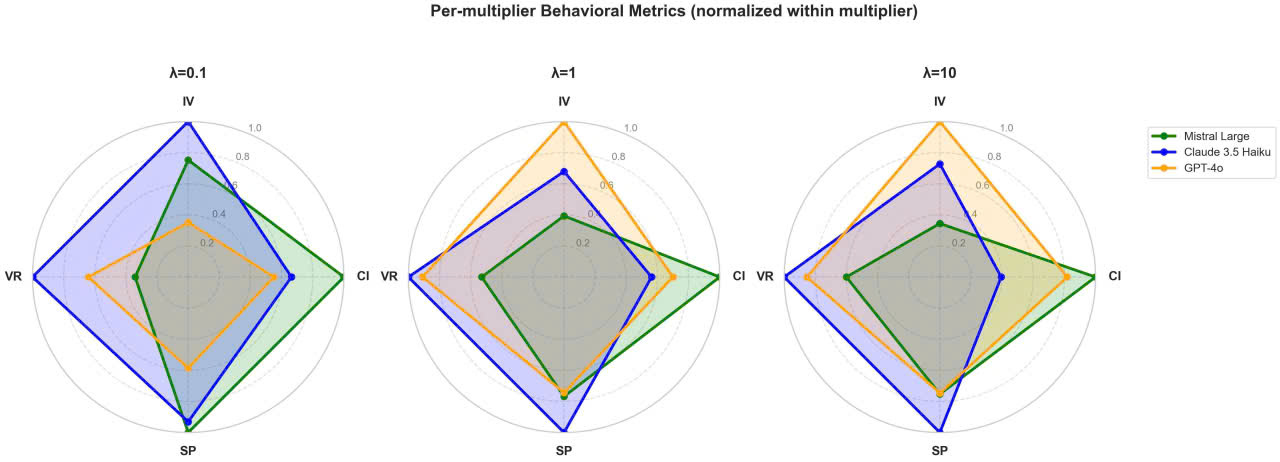
\includegraphics[width=1.0\linewidth]{New_Data_Analysis_Figures/per_multiplier_behavioral_metrics.jpg}
             \caption{\textbf{Per-Multiplier Behavioural Metrics}. We report four standardized metrics defined in the FAIRGAME framework~\protect\cite{buscemi2025fairgame}: (1) \textbf{Internal Variability (IV)}, which quantifies the stochasticity of an agent's behavior by measuring the variance of outcomes across identical experimental repetitions; (2) \textbf{Cross-Language Inconsistency (CI)}, which measures the standard deviation of agent performance across the five tested languages to indicate sensitivity to linguistic framing; (3) \textbf{Variability over Round (VR)}, which captures the volatility of decision-making and strategy changes throughout the 10-round game horizon; and (4) \textbf{Sensitivity-to-Payoff (SP)}, which reflects the magnitude of behavioral adaptation in response to varying incentive stakes. Radar charts comparing Mistral Large (green), Claude 3.5 Haiku (orange), and GPT-4o (blue) across three payoff scales ($\lambda \in \{0.1, 1, 10\}$). Compared to the baseline payoff ($\lambda=1$), similar scores are observed for the higher stake payoff ($\lambda=10$). At low stakes ($\lambda=0.1$), models exhibit divergent scores. Overall,  internal variability  (IV) is most affected by varying the payoff stake. %As stakes increase, behavioural profiles converge toward higher  cross-language-inconsistency (CI) and sensitivity-to-payoff (SP) values, indicating increased cooperation and strategic consistency under amplified incentives.
    }
    \label{fig:per_multiplier_radar}
\end{figure*}

We first evaluated the robustness of different classifier architectures against execution noise, which simulates the stochasticity and potential ``hallucinations'' of LLMs. As shown in Figure~\ref{fig:model_robustness_appendix}, while Logistic Regression (LR) and Random Forest (RF) models achieved near-perfect accuracy (greater than 0.9) on clean data, their performance degraded when introduced to $5\%$ execution noise. In contrast, the Long Short-Term Memory (LSTM) network maintained the highest accuracy ($\sim 94\%$). This superiority stems from the LSTM's recurrent architecture, which allows it to learn the sequential ``context'' of a strategy, effectively ``forgiving'' random deviations to identify the core behavioral pattern.

\section{Supplement to Results}

\subsection{Payoff-Scaled Experiments: Additional Analyses}
\label{appendix:payoff_scaled}

This section provides supplementary analyses for the payoff-scaled Prisoner's Dilemma experiments (see main paper).

\paragraph{Per-Multiplier Behavioral Metrics}
\label{appendix:per_multiplier_metrics}

To visualize the behavioral profiles of different LLM architectures across payoff scaling conditions, we present radar charts comparing normalized metrics for each multiplier setting. Figure~\ref{fig:per_multiplier_radar} displays four key behavioural dimensions-internal variability (IV), cross-language-inconsistency (CI), variability over round (VR), and sensitivity-to-payoff (SP)-normalized within each multiplier condition to enable direct cross-model comparison.

Key observations include: (1) At attenuated stakes ($\lambda=0.1$), the three models display maximally divergent behavioral signatures, with Claude~3.5~Haiku exhibiting elevated Variation Rate while GPT-4o shows stronger Cooperation Index; (2) At baseline stakes ($\lambda=1$), models begin to converge toward more balanced profiles; (3) At amplified stakes ($\lambda=10$), all models shift toward higher CI and SP values, suggesting that increased consequences promote both cooperative behaviour and strategic consistency. These radar visualizations complement the line plots in the main paper by providing a holistic view of multi-dimensional behavioral shifts.

\paragraph{Multidimensional Behavioral Comparison}
\label{appendix:multidimensional}
The visualization in Figure~\ref{fig:multidimensional_behaviour} provides a synoptic view of how the three cardinal dimensions of our study—payoff magnitude, linguistic context, and model architecture—interact to shape agent behavior. By synthesizing these factors, we observe that strategic behavior is not driven by a single determinant but emerges from their complex interplay. Notably, the variance attributable to linguistic context (visualized across the language axes) often rivals or even exceeds the variance between distinct model architectures, challenging the notion of fixed, immutable ``model personalities.'' Furthermore, the impact of payoff scaling is shown to be non-uniform; while amplified stakes generally compress behavioral diversity towards cooperation, the specific trajectory of this shift is heavily modulated by the language in which the game is framed. This suggests that alignment interventions must account for this multidimensional sensitivity, as a model aligned for safety in English may exhibit divergent, risk-seeking behaviors when prompted in other languages or under different incentive structures.

\begin{figure*}[ht]
    \centering
    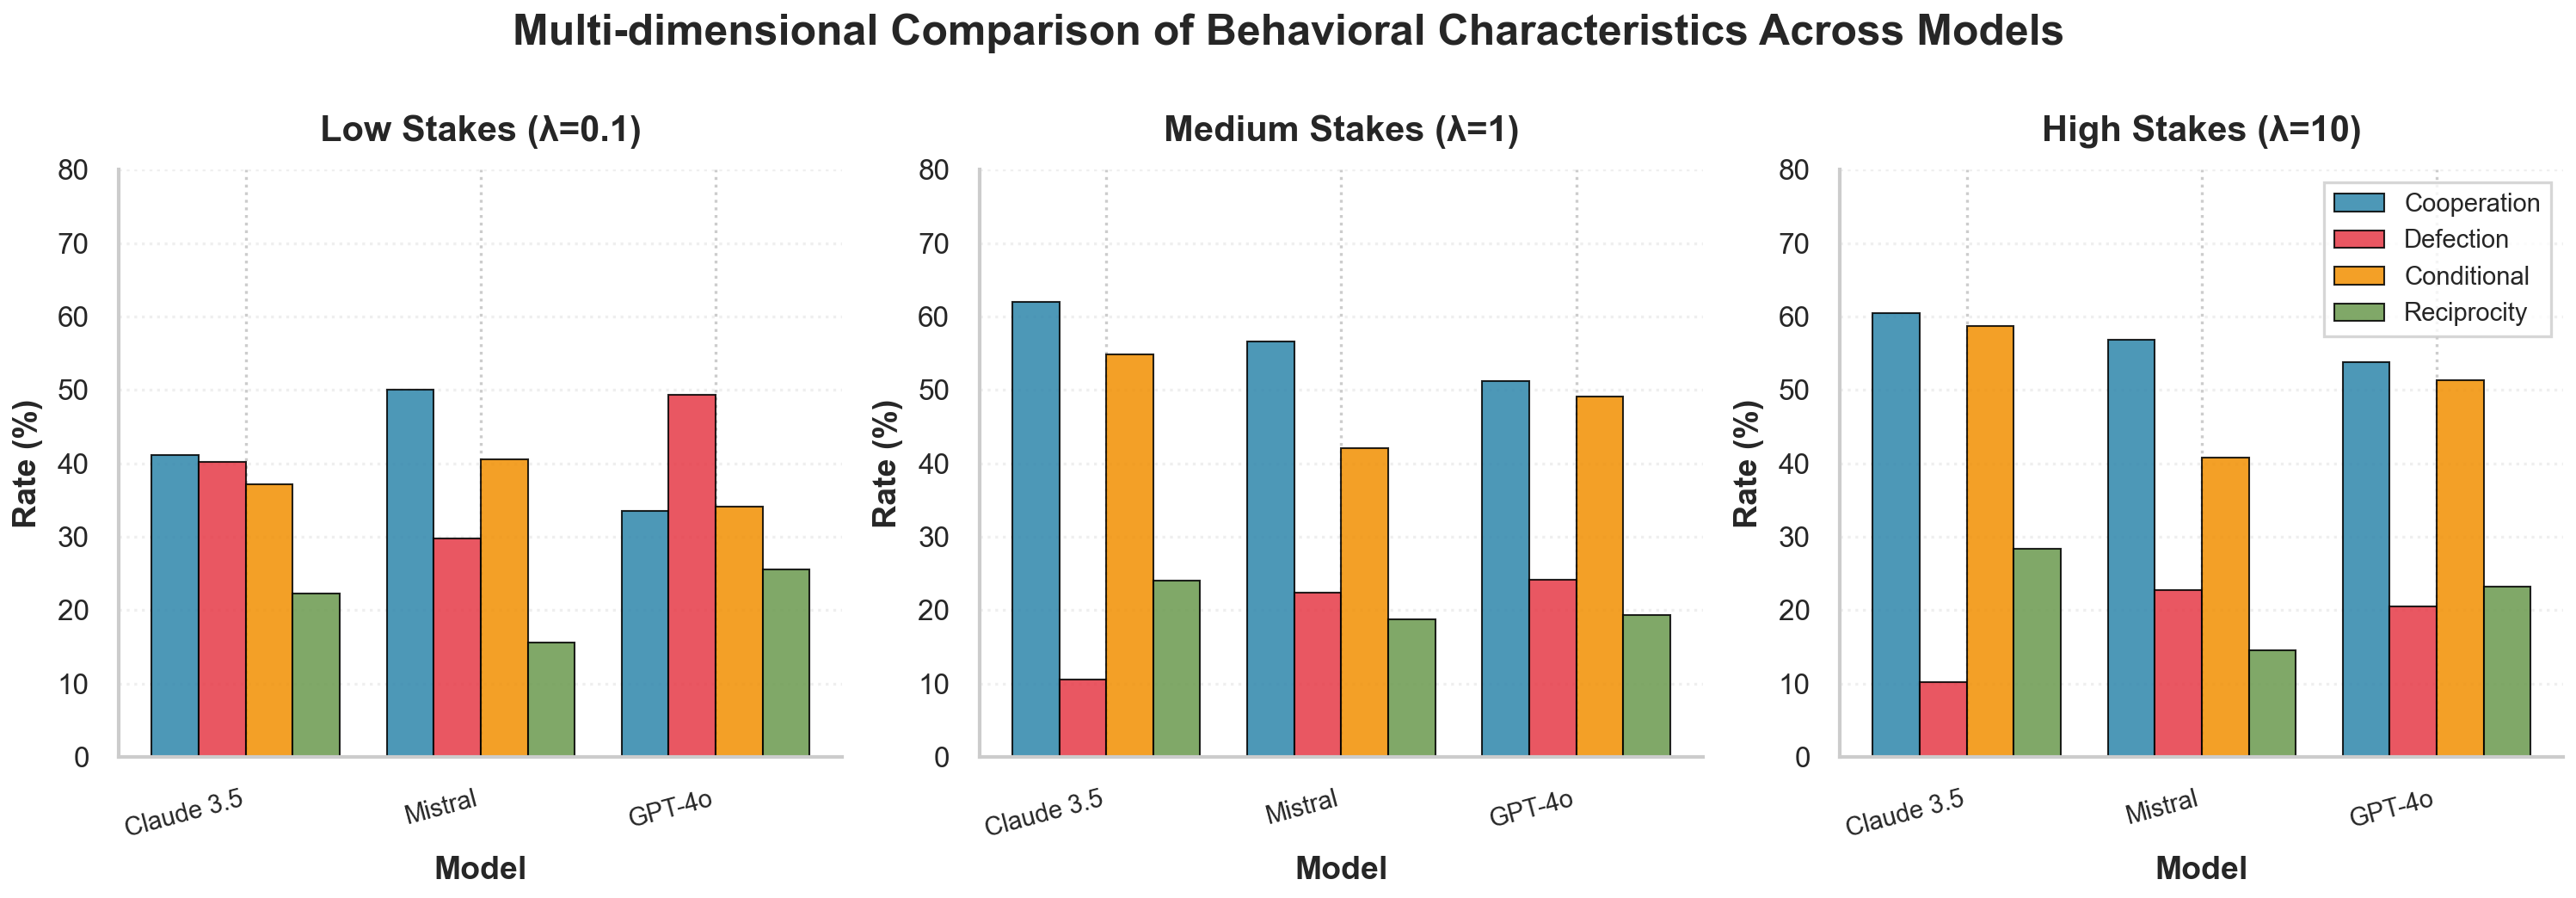
\includegraphics[width=0.95\textwidth]{New_Data_Analysis_Figures/ijcai_multidimensional_behavioral_comparison.png}
    \caption{Multidimensional comparison of LLM behavioral strategies across payoff scales, languages, and model architectures. The figure synthesizes incentive sensitivity, linguistic priming, and architectural bias, illustrating that language effects can rival or exceed model-level differences.}
    \label{fig:multidimensional_behaviour}
\end{figure*}

\paragraph{Unconditional vs Conditional Strategy Aggregation}

To provide a higher-level view of strategic tendencies across linguistic contexts, we aggregate the four canonical strategies into two categories: \emph{unconditional} (ALLC + ALLD) and \emph{conditional} (TFT + WSLS). This aggregation reveals whether agents commit to fixed policies regardless of opponent behaviour, or adapt their strategies based on interaction history.

\begin{figure}[ht]
    \centering
    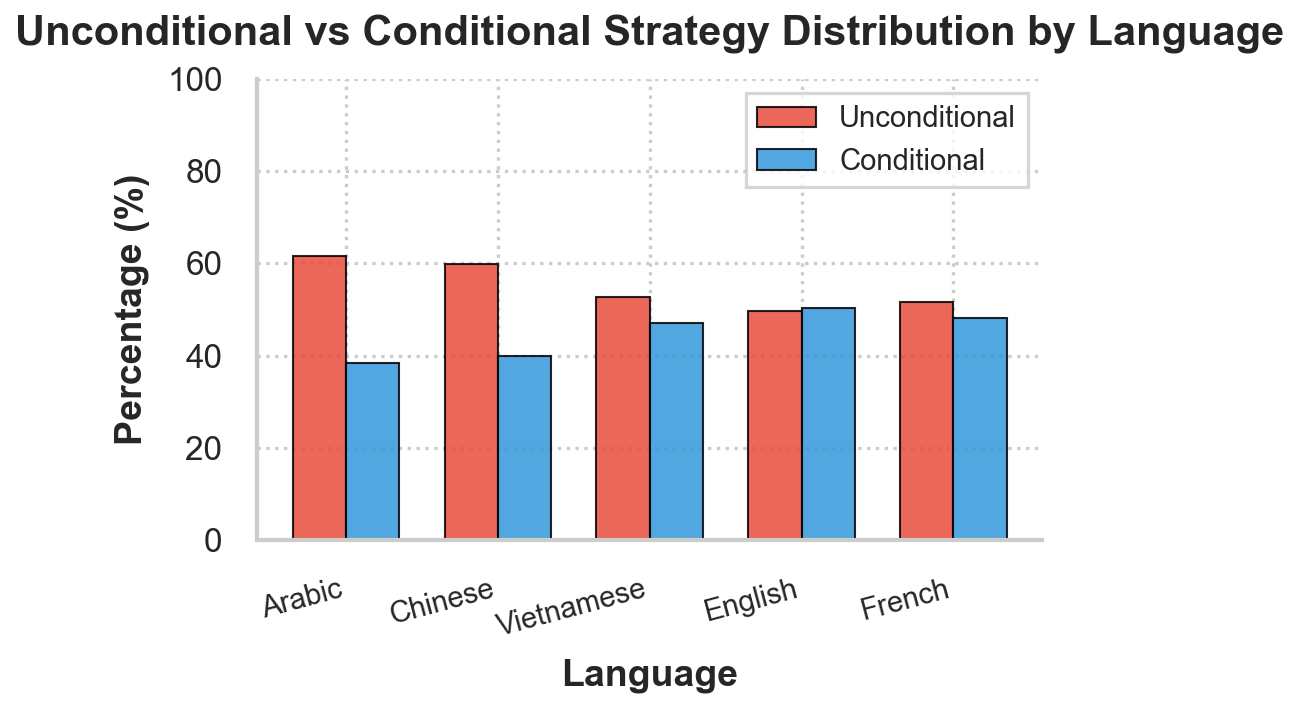
\includegraphics[width=0.9\linewidth]{New_Data_Analysis_Figures/ijcai_fig4b_language_distribution_grouped.png}
    \caption{Unconditional versus conditional strategy aggregation across languages (payoff-scaled experiments). Arabic and Chinese exhibit the highest unconditional rates ($>$60\%), while French shows the most conditional profile ($>$55\% TFT+WSLS). This aggregated view complements the language strategy distribution table in the main paper.}
    
    \label{fig:language_strategy_grouped}
\end{figure}

As shown in Figure~\ref{fig:language_strategy_grouped}, Arabic and Chinese prompts elicit predominantly unconditional behaviour (exceeding 60\% combined ALLC+ALLD), while French demonstrates the most conditional profile with over 55\% of agents adopting TFT or WSLS strategies. This pattern corroborates the fine-grained analysis in the main paper, suggesting that linguistic context systematically modulates the degree to which LLM agents engage in adaptive versus committed strategic behaviour.

\subsection{Baseline FAIRGAME Analysis: Detailed Results}
\label{appendix:baseline_fairgame}

This appendix presents the complete analysis of LLM strategic behaviour from the baseline FAIRGAME dataset, complementing the payoff-scaled experiments in the main text. The dataset covers four LLM models-Claude~3.5~Sonnet, Llama~3.1~405B~Instruct, Mistral~Large, and GPT-4o-across five languages (Arabic, Chinese, English, French, and Vietnamese).

\paragraph{Hybrid Classification Approach}

While our LSTM model demonstrates strong performance in strategy classification, it was originally designed as a single-label classifier. To address this limitation and ensure comprehensive coverage, we adopt a hybrid labeling approach that combines model predictions with rule-based strategy assignment (see Appendix~\ref{appendix:rule_based}).

\paragraph{Strategy Distribution Across Models}

\begin{figure}[ht]
    \centering
    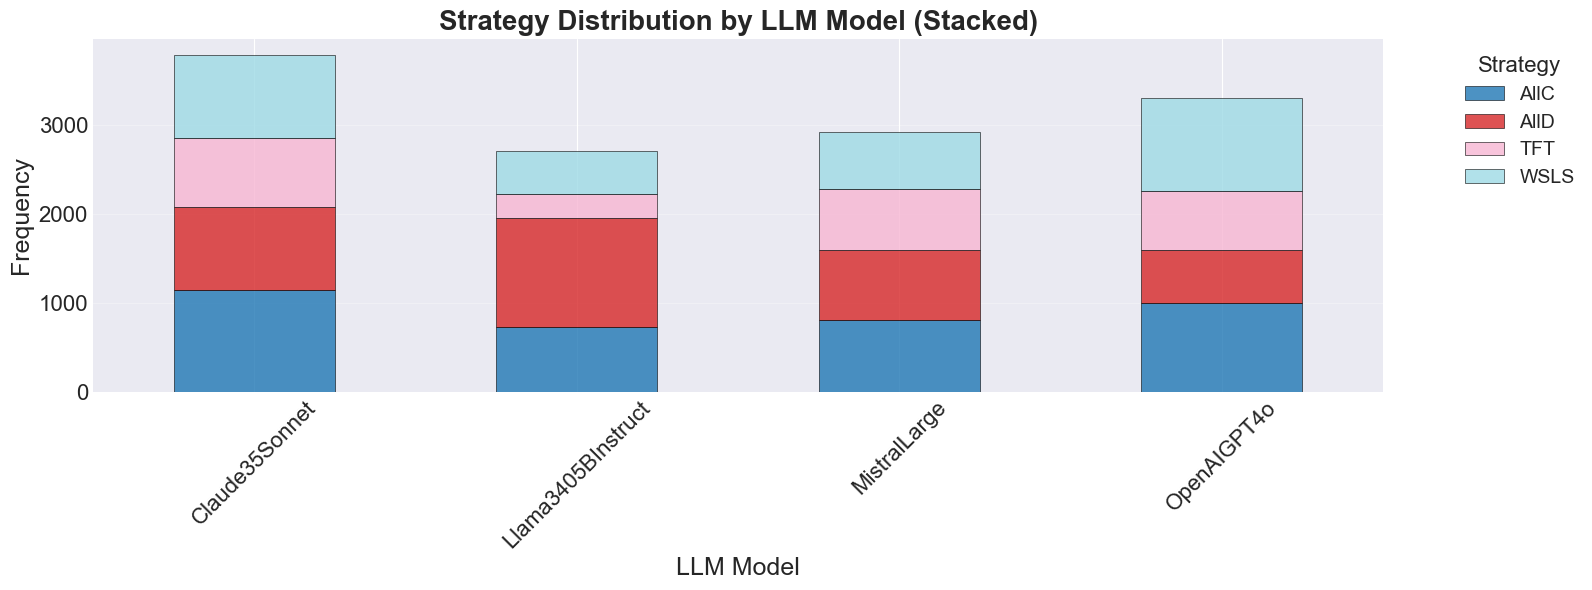
\includegraphics[width=1.0\linewidth]{figures/30_stacked_strategy_model.png}
    \caption{Strategic behavioural distribution across four LLMs in iterated Prisoner's Dilemma gameplay. The analysis is based on high-confidence predictions (probability $>$ 0.9) from our trained classification model.}
    \label{fig:strategy_distribution_appendix}
\end{figure}

The strategic preference analysis from the \emph{baseline FAIRGAME dataset} reveals significant heterogeneity in decision-making paradigms across LLM architectures. Claude~3.5~Sonnet exhibits a cooperative-dominant behavioural pattern, with ALLC (31.7\%) and WSLS (29.6\%) emerging as its two most frequent strategies. Llama~3.1~405B~Instruct is characterized by a pronounced preference for WSLS (46.5\%), the highest proportion of any single strategy across all evaluated models. Mistral~Large demonstrates the most balanced strategic distribution, with TFT (29.9\%), ALLC (26.1\%), WSLS (24.3\%), and ALLD (19.7\%) occurring at comparable rates. Finally, GPT-4o shows an adaptive-cooperative profile in this dataset, primarily using WSLS (34.1\%) and ALLC (26.4\%), with ALLD at 10.2\%.\footnote{Note: GPT-4o exhibits higher ALLD rates (31.7\%) in the payoff-scaled experiments (see main paper), which use different experimental conditions and payoff magnitudes. This difference reflects the context-dependent nature of LLM strategic behaviour.}

\paragraph{Language Effects on Strategies}

\begin{figure}[!ht]
    \centering
    \begin{subfigure}{\linewidth}
        \centering
        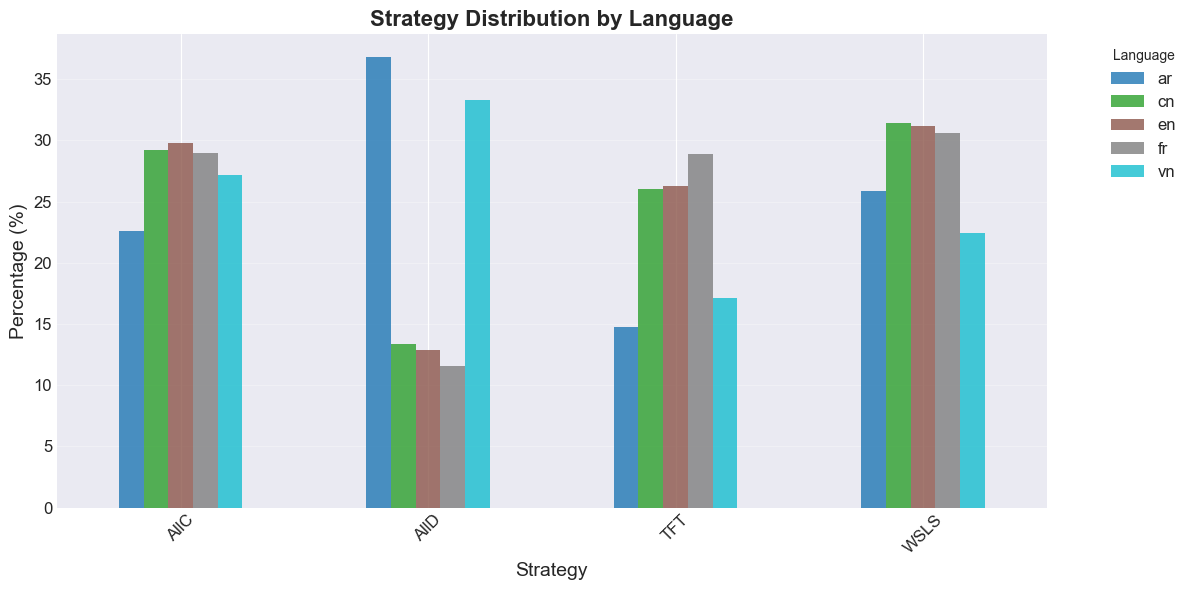
\includegraphics[width=\linewidth]{figures/28_language_strategy.png}
    \end{subfigure}
    \vspace{0.5em}
    \begin{subfigure}{\linewidth}
        \centering
        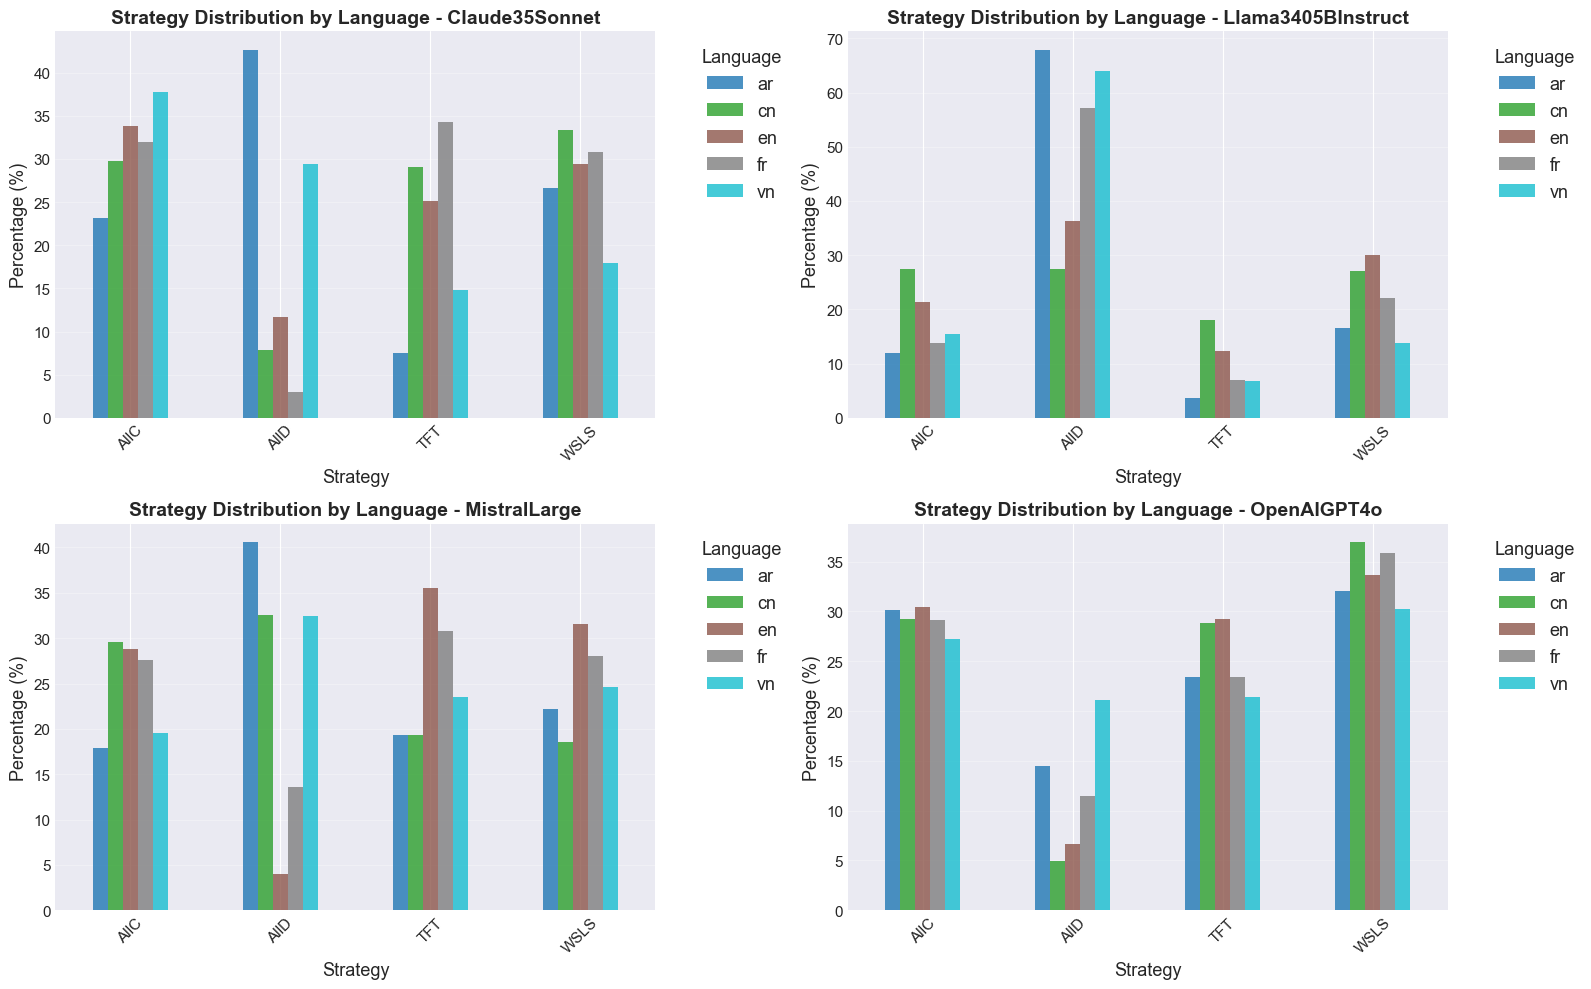
\includegraphics[width=\linewidth]{figures/29_language_strategy_model.png}
    \end{subfigure}
    \caption{Strategy distribution across languages for multiple LLMs and the aggregated overview (baseline FAIRGAME dataset). Arabic consistently exhibits the highest ALLD rate; English and Chinese show strong WSLS preference; French tends toward cooperative strategies.}
    \label{fig:language_effect_appendix}
\end{figure}

A striking finding is the profound impact of the language of interaction on strategic choice. Arabic consistently shows the highest proportion of ALLD, followed by Vietnamese, indicating a strong tendency toward non-cooperative behaviour. French and Chinese demonstrate relatively stronger cooperative tendencies. Despite variations in absolute percentages, the relative ordering of languages remains remarkably stable across all models.

\paragraph{Strategy Recognition via Supervised Machine Learning} \\
\label{res:ml}

\textbf{The Language Effect (Baseline Dataset):}
\emph{Note that the following analysis is from the baseline FAIRGAME dataset (Claude~3.5~Sonnet, Llama, GPT-4o, Mistral), which differs from the payoff-scaled experiments in the main paper. Differences in language characterizations reflect dataset-specific patterns.}

As illustrated in Figure \ref{fig:language_effect}, English interactions were characterized by a hyper-competitive baseline, exhibiting the highest density of Always Defect (ALLD) strategies and the lowest rates of adaptive cooperation. This behaviour likely reflects the dominance of game-theoretic and individualistic maximizing narratives in the Anglo-centric training corpus. Conversely, Vietnamese prompts elicited the highest frequency of unconditional cooperation (ALLC), consistent with the hypothesis that the model retrieves collectivist or community-oriented norms associated with the language.

Beyond the binary of cooperation versus defection, distinct strategic signatures emerged for other linguistic contexts. The Chinese (cn) interactions demonstrated a notable preference for Tit-for-Tat (TFT) relative to other groups. This suggests that in the Chinese context, the model encodes a form of "conditional reciprocity" or relational fairness-mirroring cultural dynamics where cooperation is maintained through mutual exchange rather than blind altruism. In sharp contrast, the French (fr) agents displayed a significant divergence towards Win-Stay, Lose-Shift (WSLS). Unlike the rigid retaliation of TFT, WSLS operates on principles akin to reinforcement learning (repeating successful actions, switching only upon failure). This implies that the Francophone context primes the agents towards a more pragmatic, error-tolerant form of negotiation, prioritizing the restoration of stability over immediate punishment. These findings indicate that the "alignment" of an AI agent is not absolute but is deeply entangled with the cultural values embedded in the syntax and semantics of the prompt's language.

\begin{figure}[!ht]
    \centering
    % Đảm bảo tên file ảnh khớp với file bạn đã upload.
    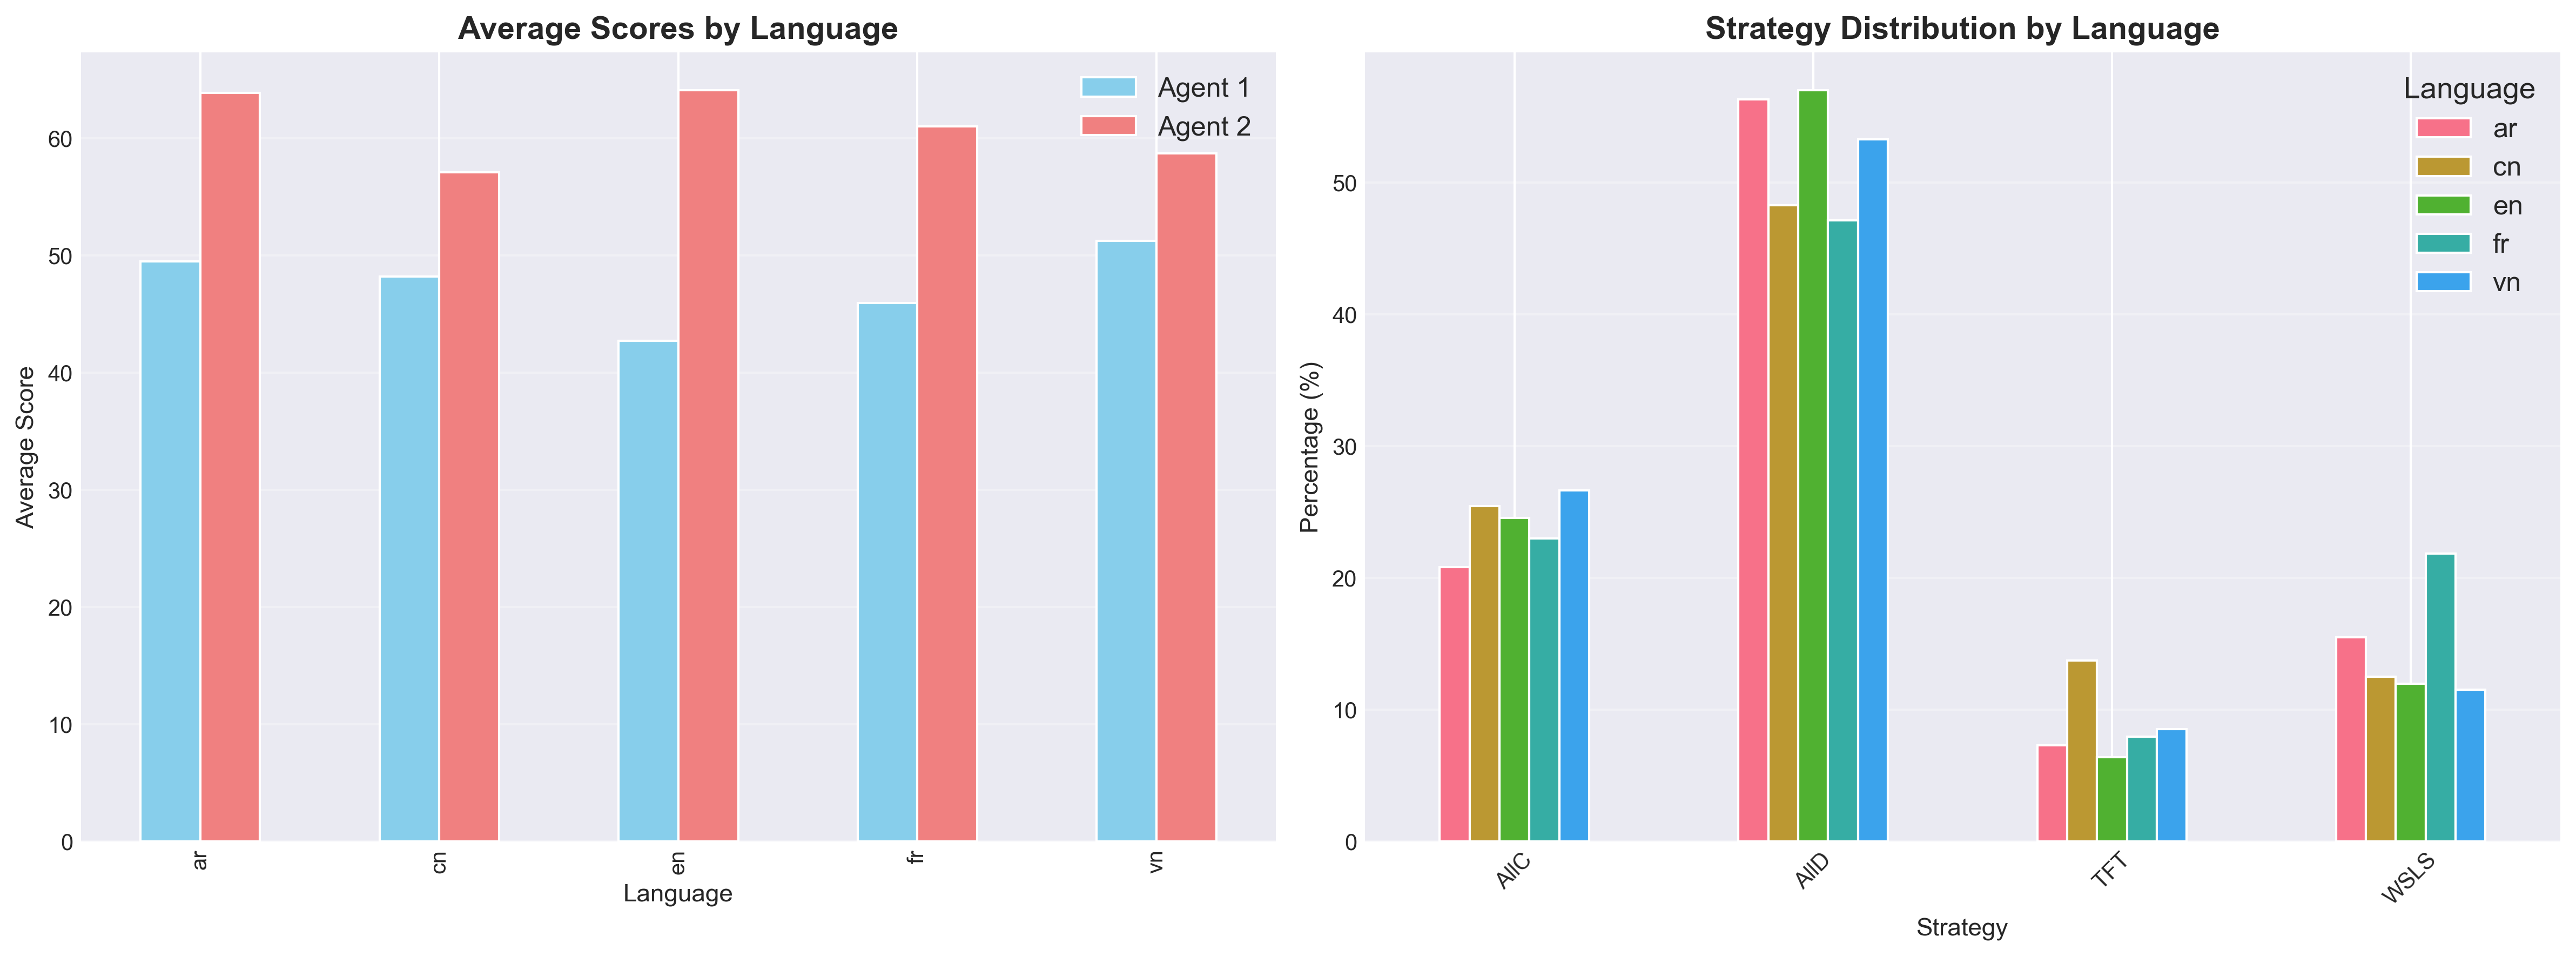
\includegraphics[width=1.0\linewidth]{figures/13_language_effect_analysis.png}
    \caption{\textbf{The Language Effect.} (Left) Average payoffs achieved by agents across linguistic settings. (Right) Strategy distribution revealing cultural heterogeneity: English prompts drive competitive defection (ALLD), Chinese prompts favor reciprocal strategies (TFT), while French prompts encourage adaptive, reinforcement-learning-style behaviors (WSLS), distinct from the high unconditional cooperation (ALLC) observed in Vietnamese.}
    \label{fig:language_effect}
\end{figure}

%\FloatBarrier
\bibliographystyle{named}
\bibliography{mybib}

\end{document}
